This is the second day! Presented our imbalanced learning work, and attended a few keynotes.

\subsection{Special session on intelligent data mining}

\subsubsection{Understanding Multilingual Communities through Analysis of Code-switching Behaviors in Social Media Discussions}

$\ra$ Research interests: twitter discuss with replies that are  multilingual. \\

$\ra$ To understand why people are changing languages in tweets replies.

datasets are human tagged, to identify whether a reply has a complete sentence in a language, and score the relevance of the reply.

\subsubsection{Explainable Visualization for interactive exploration of CNN on Wikipedia Vandal Detection}

Focused on explainable machine learning using visualization. Previous works that try to be white-box are on neuron-level which are not intuitive for layman.

\spacerule

\subsection{IEEE BigData Cup Challenge}

\subsubsection{Emotion detection using EEG signal with CNN}

Dataset: DEAP dataset, a public  dataset for emotion;\\

Classifier: SVM and CNN, interestingly, CNN is way worse  than SVM as there  are not  enough data for training a better CNN.\\

$\ra$ use  data augmentation to  increase  the  training dataset size by generating artificial data samples.\\

Data augmentation: add Gaussian noise (does not change amplitude data).\\

Data augmentation and  data  reshape has increased  the performance of  CNN tremendously, from nearly 0.65 to 0.96 (accuracy)\\

\begin{figure}[ht!]
    \centering
    \includegraphics[width=120mm]{images/eeg.png}
    \caption{EEG feature extraction}
    \label{fig:eeg}
\end{figure}

\spacerule

\subsection{Keynote 1: Federated Recommendation}

\label{section: keynote1}

The speaker is Qiang Yang who is from the WeBank and Hong Kong University of Science and Technology.\\

\note{In recommender system, the more data the better system. Through web crawling, business contract, we can have more data sources. But the question is "is this approach sustainable?"}

\note{In health care systems, ``federated learning" is pretty important as it protects the privacy of clinical data. This could be another research direction in the future and the speaker says there are a lot of low-hanging fruit in this research area}

Conventional machine learning requires centralizing the training data on one machine or in a data center. And Google has built one of the most secure and robust cloud infrastructures for processing this data to make our services better. Now for models trained from user interaction with mobile devices, we're introducing an additional approach: Federated Learning. 

\ddef{Federated learning}{Federated Learning is a machine learning setting where the goal is to train a high-quality centralized model with training data distributed over a large number of clients each with unreliable and relatively slow network connections.}

\ddef{data silos}{data islands that are shared between research entities as security issues or other reasons.}

$\ra$ The federated learning is good for protecting data privacy as the training process is decentralized.\\


{\bf FATE}\footnote{\url{https://github.com/FederatedAI/FATE}} is a open-source framework for industrial federated recommender system

\subsubsection{Keynote 2: the new science of cause and effect, with reflections on data science and artificial intelligence}

The speaker is Judea Pearl. 

{\bf Why data science needs a new engine, to answer causal questions.}\\

The seven tools of causal inference

\begin{itemize}
    \item Encode causal info in transparent and testable way.
    \item Predicting the effects of actions and policies.
    \item Computing counterfactuals and finding causes of effects
    \item Computing direct and indirect effects (Mediation)
    \item Integrating data from diverse sources
    \item Recovering from missing data
    \item Discovering causal relations from data (growing field)
\end{itemize}

\remark{Causal relation discovery is a growing field and we can check in the literature from CMU and UCLA on the related work.}

\remark{current science build on equality(y=ax equals to x = y/a), hence cannot answer uni-directional questions, e.g., causal questions}

\begin{figure}[htbp!]
    \centering
    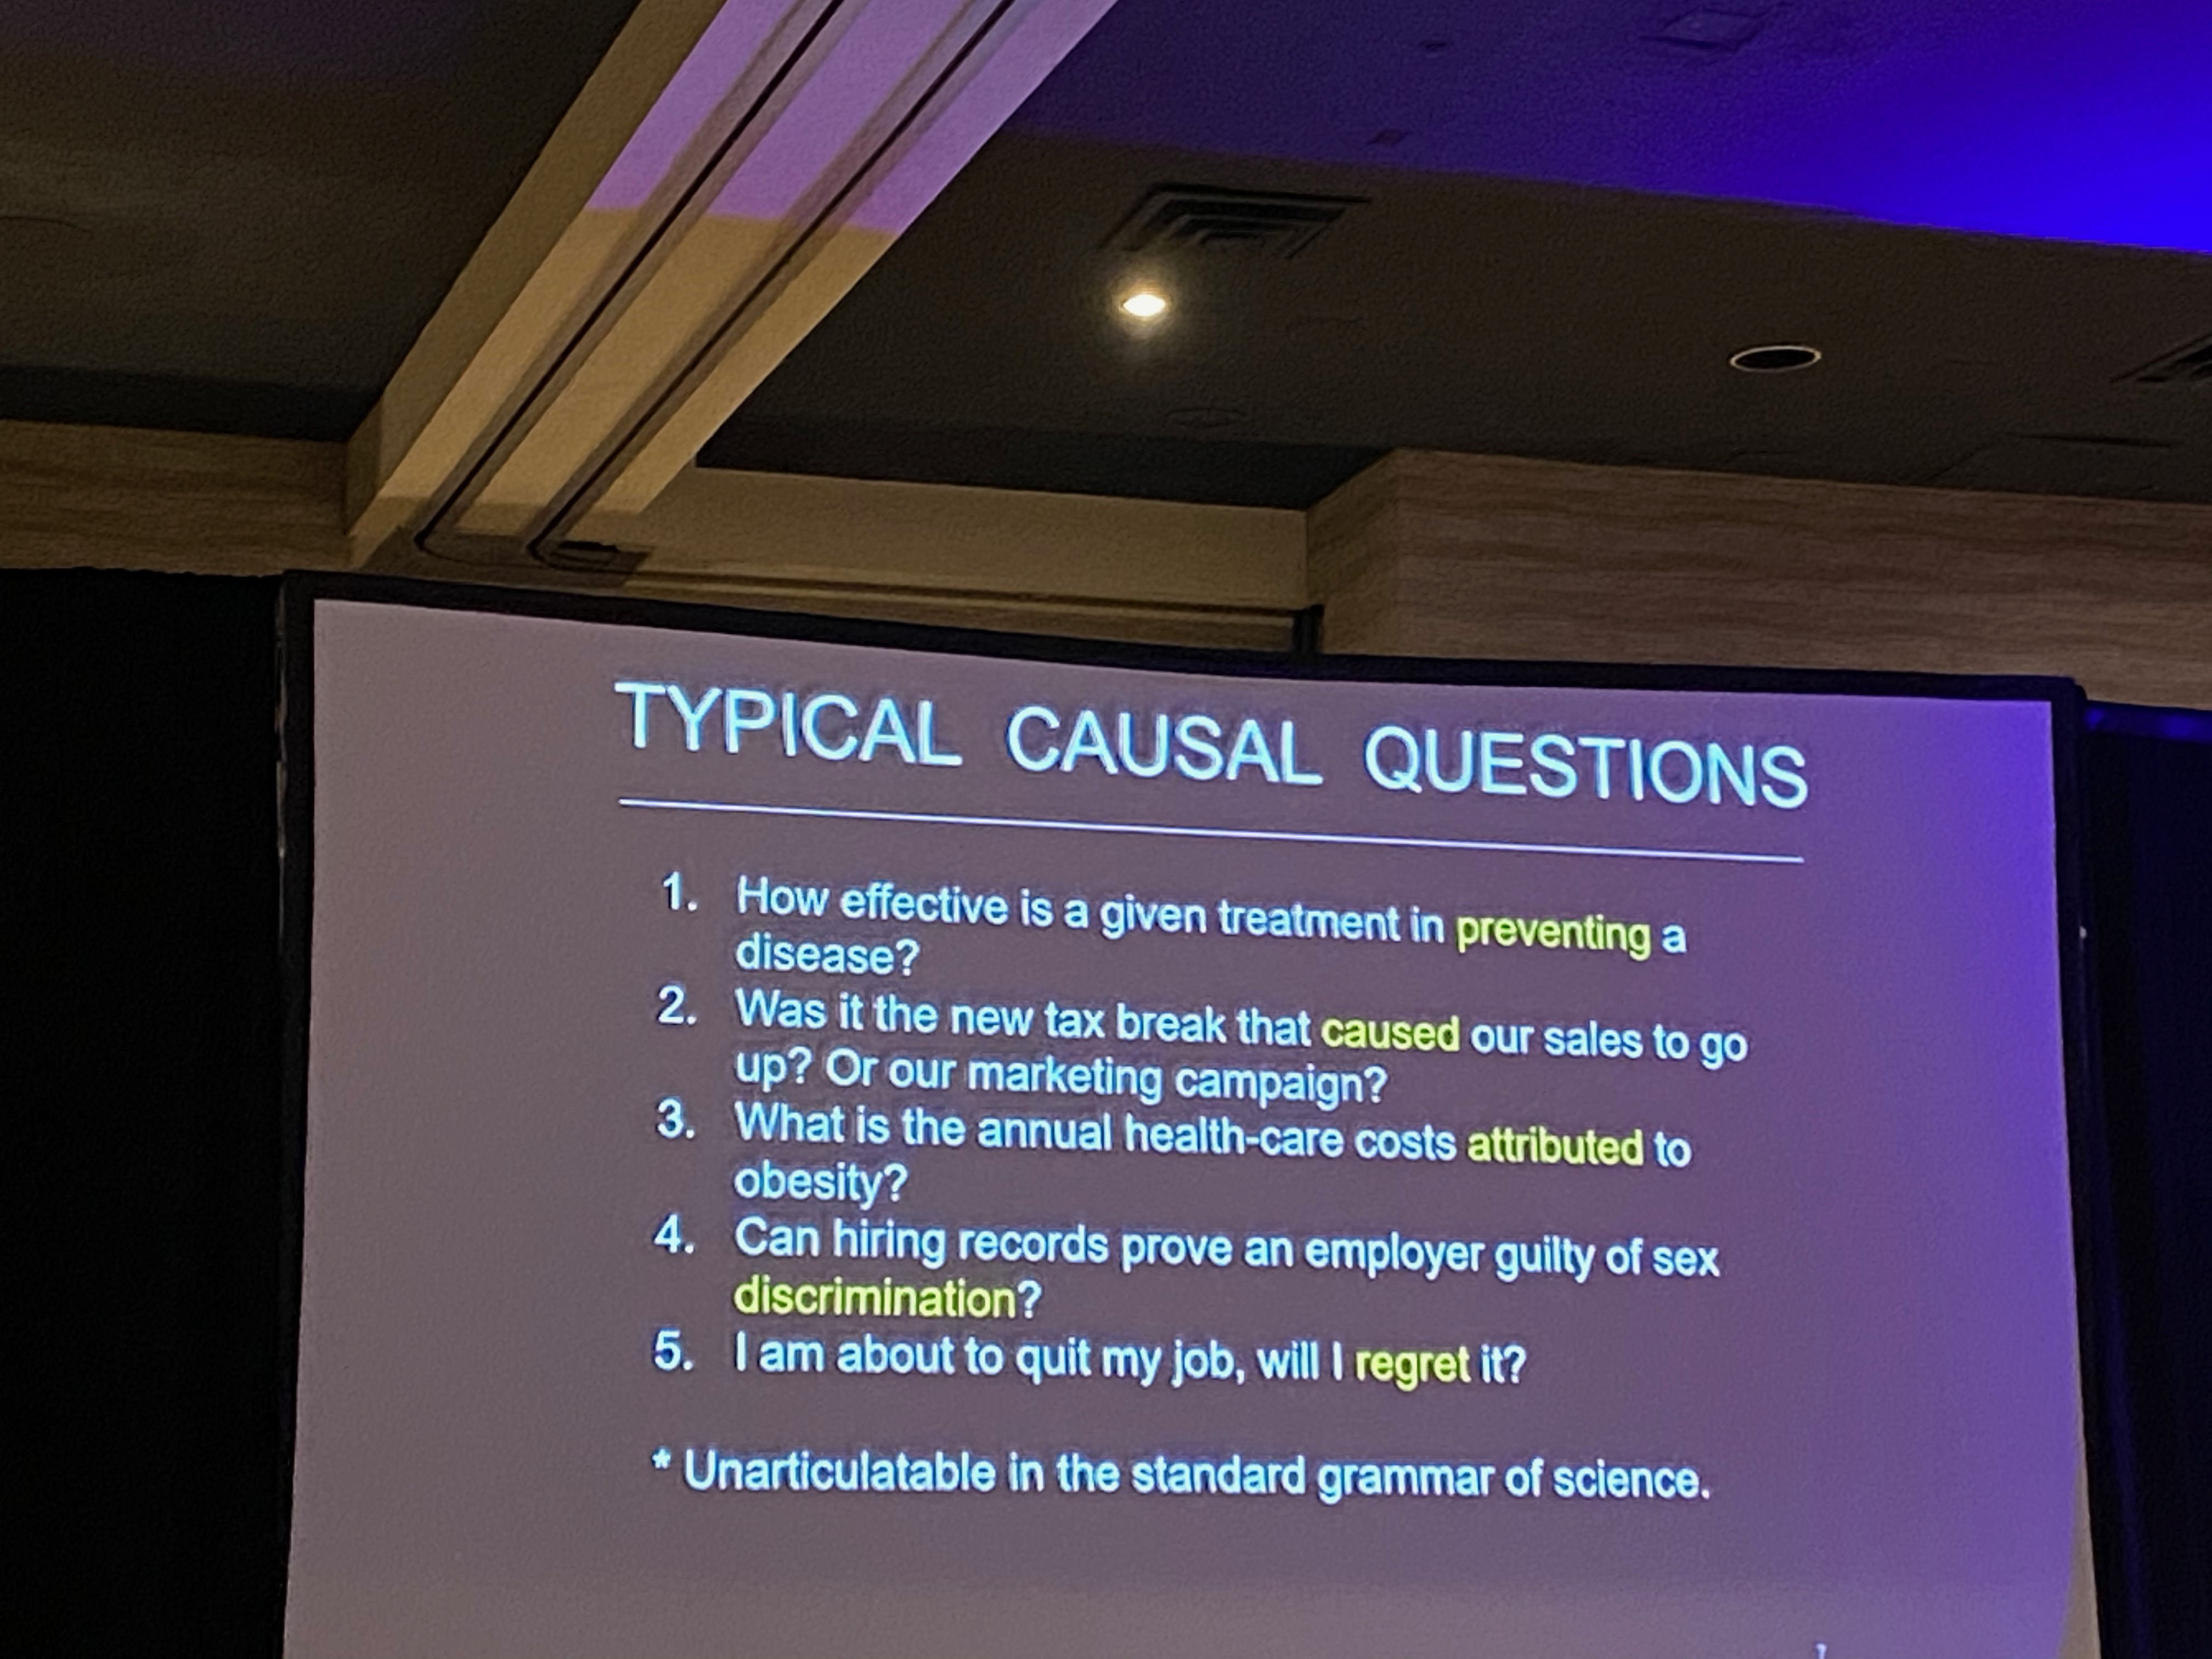
\includegraphics[width=120mm]{images/causal_questions.png}
    \caption{Causal questions}
    \label{fig:causal_questions}
\end{figure}

\begin{figure}[htbp!]
    \centering
    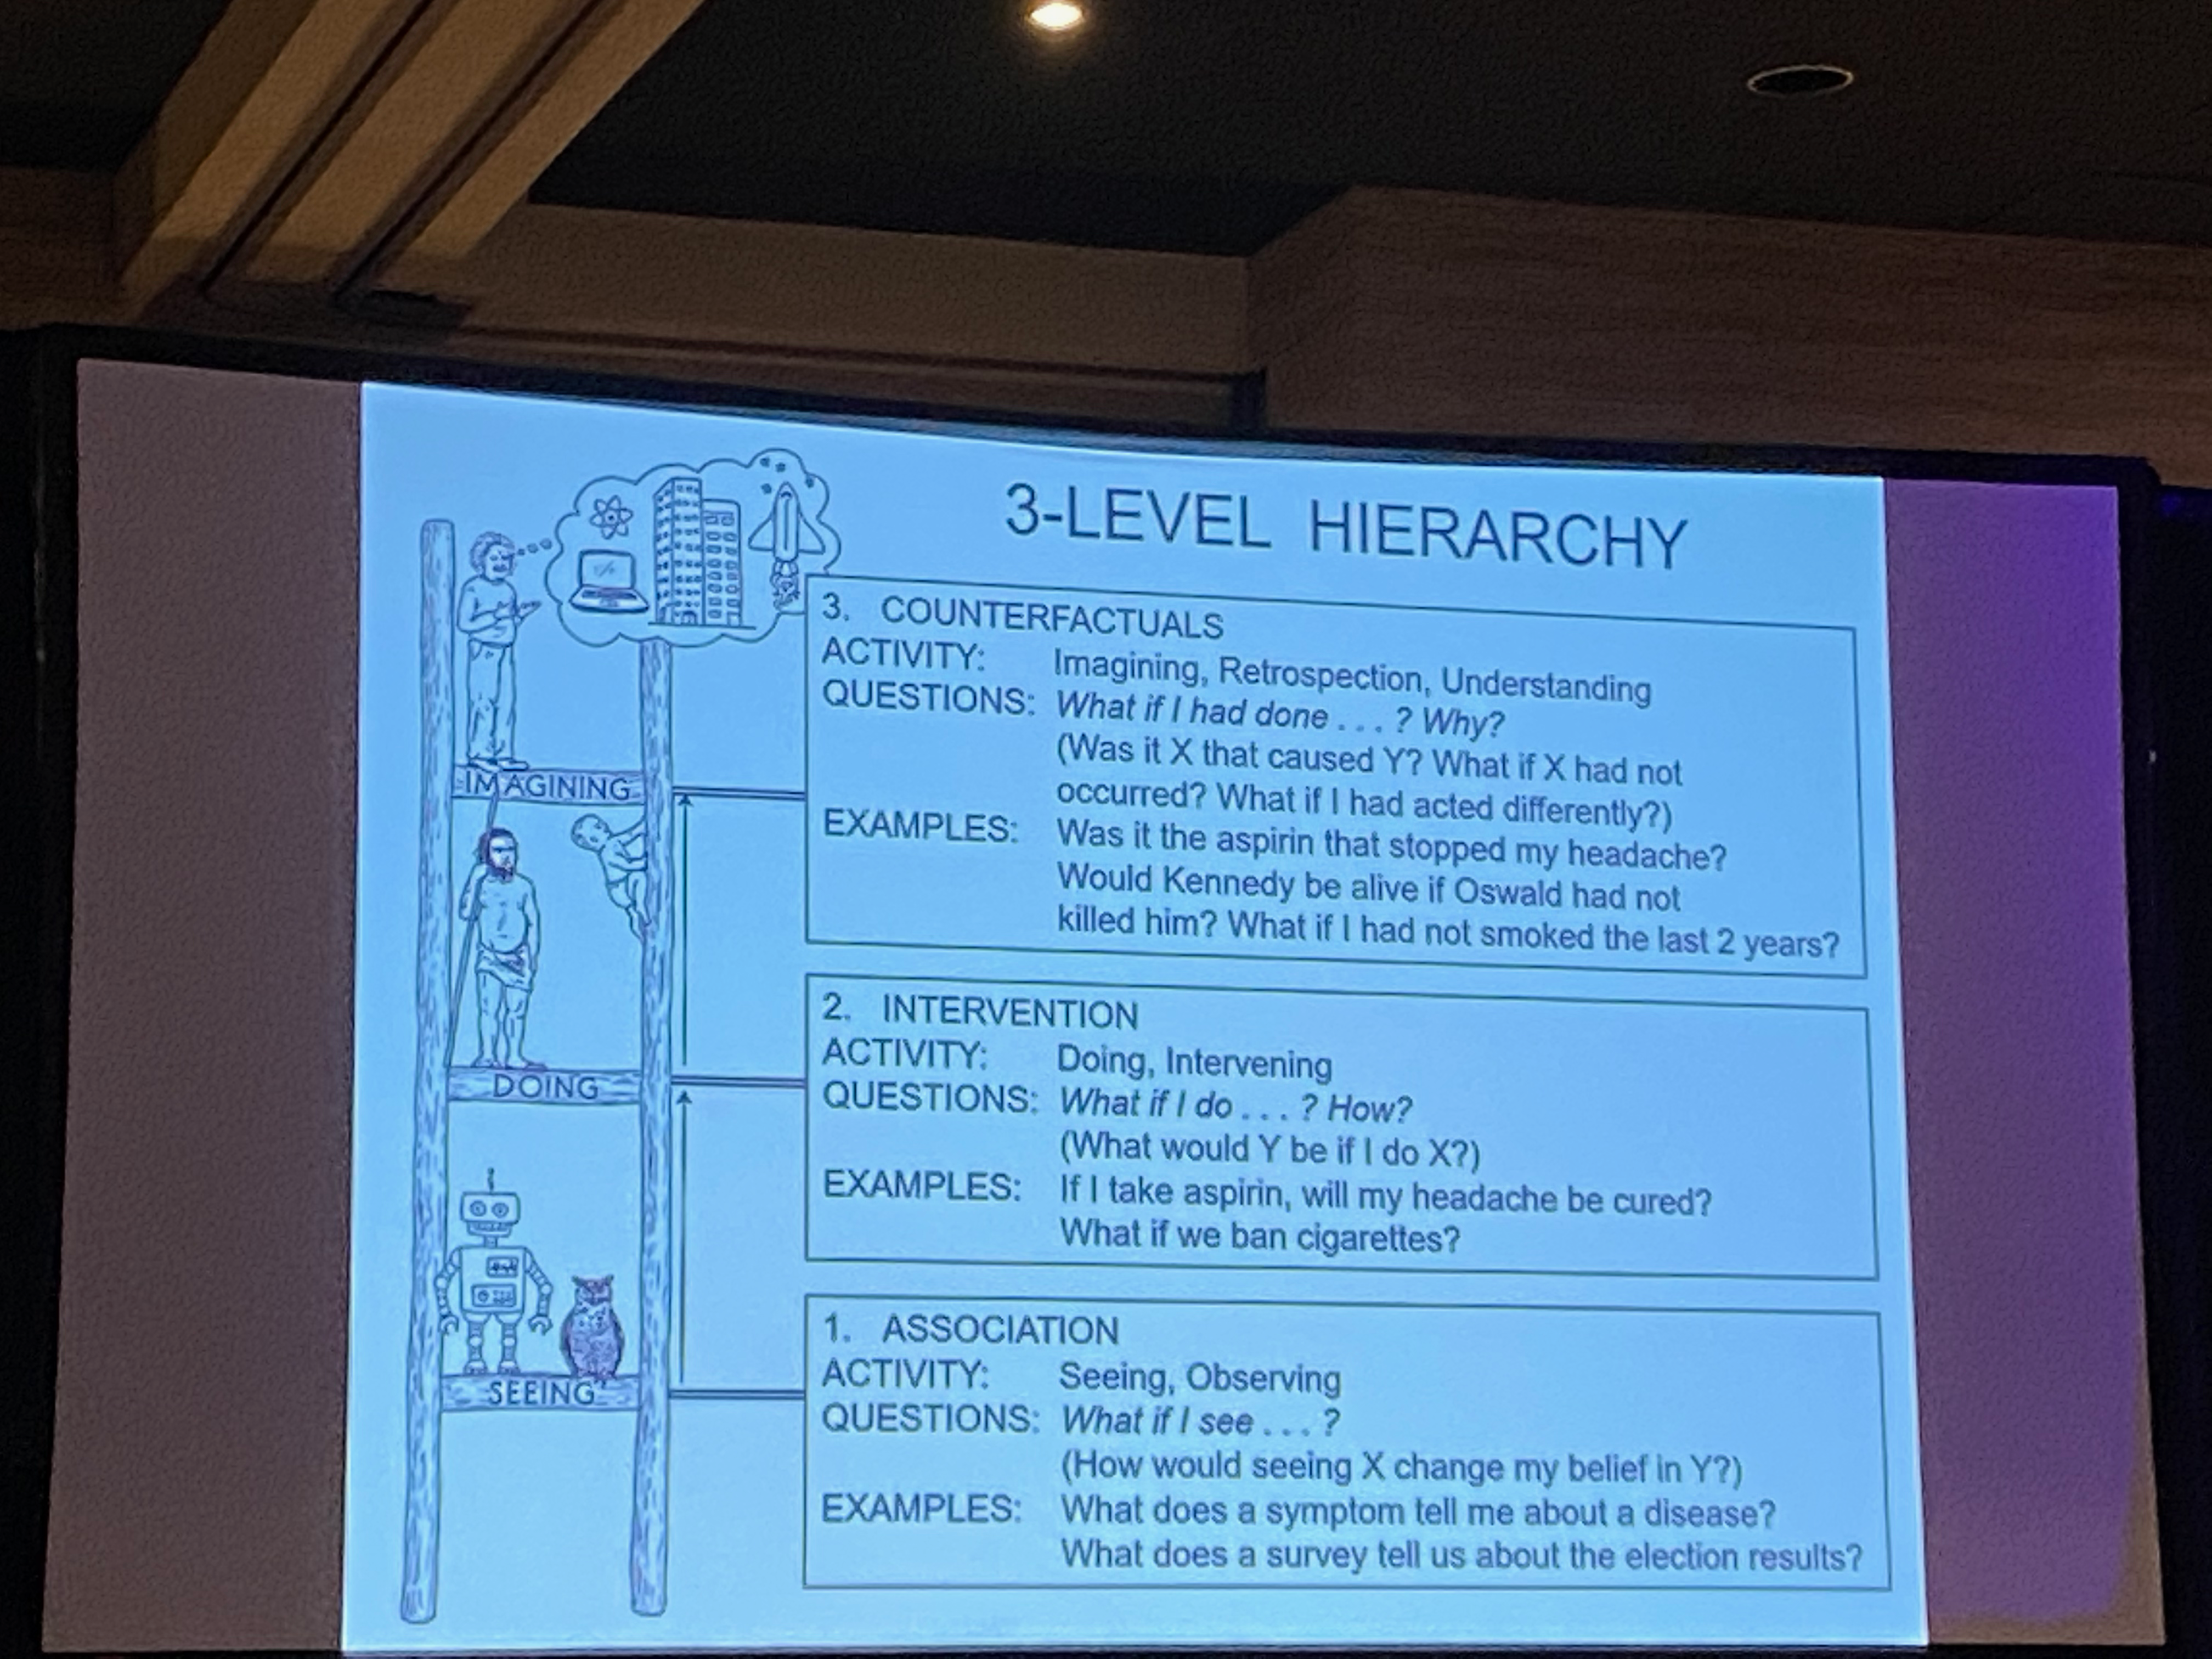
\includegraphics[width=120mm]{images/causal_ladder.png}
    \caption{3-level Causal ladder}
    \label{fig:causal_laddar}
\end{figure}

\idea{Can we answer the question: how much data missing is too much using Mohan and Pearl's work}



\spacerule